\documentclass[10pt,journal,compsoc]{IEEEtran}

\usepackage{amsmath}
\usepackage{graphicx}
\usepackage{algorithm}
\usepackage{algpseudocode}
\usepackage{listings}
\usepackage{xcolor}
\usepackage{hyperref}

\definecolor{codegreen}{rgb}{0,0.6,0}
\definecolor{codegray}{rgb}{0.5,0.5,0.5}
\definecolor{codepurple}{rgb}{0.58,0,0.82}
\definecolor{backcolour}{rgb}{0.95,0.95,0.95}

\lstdefinestyle{mystyle}{
    backgroundcolor=\color{backcolour},   
    commentstyle=\color{codegreen},
    keywordstyle=\color{codepurple},
    numberstyle=\tiny\color{codegray},
    stringstyle=\color{codegreen},
    basicstyle=\ttfamily\footnotesize,
    breakatwhitespace=false,         
    breaklines=true,                 
    captionpos=b,                    
    keepspaces=true,                 
    numbers=left,                    
    numbersep=5pt,                  
    showspaces=false,                
    showstringspaces=false,
    showtabs=false,                  
    tabsize=2
}

\lstset{style=mystyle}

\begin{document}

\title{Multiclass Classification of Handwritten Digits Using Softmax Regression on the MNIST Dataset}

\author{
\IEEEauthorblockN{Deepak Silaych, Parul Khicha, Shubham Garg\\
Department of Civil Engineering\\
Indian Institute of Technology Bombay\\
Mumbai, India}
}

\maketitle

\begin{abstract}
This paper presents an implementation of multiclass classification using softmax regression applied to the MNIST handwritten digit dataset. We develop a complete pipeline for data loading, preprocessing, model training with the Adam optimizer, and evaluation. Our implementation incorporates key techniques such as regularization, learning rate decay, and early stopping to enhance model performance. The results demonstrate the effectiveness of softmax regression for digit classification, achieving competitive accuracy rates while maintaining computational efficiency. We analyze model performance through multiple evaluation metrics, including confusion matrices and example predictions. Our findings highlight both the strengths and limitations of linear classification methods for image recognition tasks.
\end{abstract}

\begin{IEEEkeywords}
MNIST, softmax regression, multiclass classification, machine learning, Adam optimizer, early stopping
\end{IEEEkeywords}

\section{Introduction}
Handwritten digit recognition remains a fundamental benchmark problem in computer vision and machine learning. The MNIST dataset \cite{lecun1998gradient}, containing 70,000 grayscale images of handwritten digits, has been widely used for developing and comparing classification algorithms. Despite advances in deep learning, traditional methods such as logistic regression continue to provide valuable baselines and insights into the classification process.

In this paper, we implement a multiclass logistic regression classifier using the softmax activation function, commonly known as softmax regression. We apply this approach to the MNIST dataset and develop a complete pipeline that includes data loading, preprocessing, model training, and evaluation. Our implementation incorporates several optimization techniques:

\begin{itemize}
    \item Adam optimizer for efficient training
    \item L2 regularization to prevent overfitting
    \item Learning rate adaptation for improved convergence
    \item Early stopping based on validation performance
\end{itemize}

We provide a detailed analysis of the model's performance through various evaluation metrics, including accuracy, confusion matrices, and visualizations of example predictions. Our work demonstrates the effectiveness of softmax regression for digit classification and provides insights into the strengths and limitations of linear classification methods for image recognition tasks.

\section{Methodology}
\subsection{Problem Formulation}
Given an input image $\mathbf{x} \in \mathbb{R}^d$, where $d$ is the number of pixels (in the case of MNIST, $d = 28 \times 28 = 784$), our goal is to classify the image into one of $K$ classes (for MNIST, $K = 10$, corresponding to the digits 0-9). We formulate this as a multiclass classification problem and use softmax regression to estimate the probability distribution over the possible classes.

\subsection{Softmax Regression}
Softmax regression extends logistic regression to the multiclass setting. The model computes the probability of each class $k$ given the input $\mathbf{x}$ as:

\begin{equation}
P(y = k | \mathbf{x}) = \frac{e^{\mathbf{w}_k^T \mathbf{x} + b_k}}{\sum_{j=1}^{K} e^{\mathbf{w}_j^T \mathbf{x} + b_j}}
\end{equation}

where $\mathbf{w}_k \in \mathbb{R}^d$ is the weight vector for class $k$, and $b_k \in \mathbb{R}$ is the bias term for class $k$.

\subsection{Loss Function}
We use the cross-entropy loss function, which is the negative log-likelihood of the true class probabilities. For a single example $(\mathbf{x}, \mathbf{y})$, where $\mathbf{y}$ is a one-hot encoded vector of the true class, the loss is:

\begin{equation}
\mathcal{L}(\mathbf{w}, \mathbf{b}; \mathbf{x}, \mathbf{y}) = -\sum_{k=1}^{K} y_k \log(P(y = k | \mathbf{x}))
\end{equation}

To prevent overfitting, we add L2 regularization to the loss function:

\begin{equation}
\mathcal{J}(\mathbf{w}, \mathbf{b}) = \frac{1}{m} \sum_{i=1}^{m} \mathcal{L}(\mathbf{w}, \mathbf{b}; \mathbf{x}^{(i)}, \mathbf{y}^{(i)}) + \frac{\lambda}{2m} \sum_{j=1}^{K} \|\mathbf{w}_j\|_2^2
\end{equation}

where $m$ is the number of training examples, and $\lambda$ is the regularization parameter.

\subsection{Optimization}
We use the Adam optimizer to optimize the parameters \(\mathbf{w}\) and \(\mathbf{b}\). Adam is an adaptive learning rate optimization algorithm that's been designed specifically for training deep neural networks. It combines the advantages of two other extensions of stochastic gradient descent: AdaGrad and RMSProp.

The update rules for the parameters are:

\begin{align}
\mathbf{w}_k &\leftarrow \mathbf{w}_k - \alpha \nabla_{\mathbf{w}_k} \mathcal{J} \\
b_k &\leftarrow b_k - \alpha \nabla_{b_k} \mathcal{J}
\end{align}

where \(\alpha\) is the learning rate.

\subsection{Implementation Details}
Our implementation includes the following components:

\begin{enumerate}
    \item \textbf{Data Loading and Preprocessing:} We load the MNIST dataset from CSV files and normalize the pixel values to the range [0, 1]. We split the training data into training and validation sets.
    
    \item \textbf{One-Hot Encoding:} We convert the class labels to one-hot encoded vectors for training.
    
    \item \textbf{Adam Optimizer:} We implement the Adam optimizer for efficient training.
    
    \item \textbf{Learning Rate Decay:} We use an exponential decay schedule for the learning rate to improve convergence.
    
    \item \textbf{Early Stopping:} We monitor the validation loss and stop training if it does not improve for a specified number of iterations.
    
    \item \textbf{Evaluation:} We evaluate the model's performance on validation and test sets using accuracy metrics and visualizations.
\end{enumerate}

\section{Experimental Setup}
\subsection{Dataset}
We use the MNIST dataset, which consists of 60,000 training images and 10,000 test images of handwritten digits. Each image is a 28×28 grayscale image, represented as a vector of 784 features (pixel values). We further split the training set into 54,000 training examples and 6,000 validation examples.

\subsection{Preprocessing}
We normalize the pixel values to the range [0, 1] by dividing by 255. This normalization helps improve the convergence of the optimization algorithm.

\subsection{Hyperparameters}
We use the following hyperparameters for our experiments:
\begin{itemize}
    \item Initial learning rate ($\alpha$): 0.1
    \item L2 regularization parameter ($\lambda$): 0.01
    \item Batch size: 256
    \item Maximum number of iterations: 2000
    \item Patience for early stopping: 10
    \item Learning rate decay rate: 0.95
    \item Learning rate decay steps: 100
\end{itemize}

\section{Results and Discussion}
\subsection{Training Convergence}
Fig. 1 shows the training and validation loss over the course of training. The loss decreases steadily during the initial iterations and then begins to plateau. The gap between the training and validation loss is small, indicating that the model is not overfitting significantly. The learning rate decay and early stopping mechanisms help ensure stable convergence and prevent the model from overfitting.

\begin{figure}[htbp]
\centering
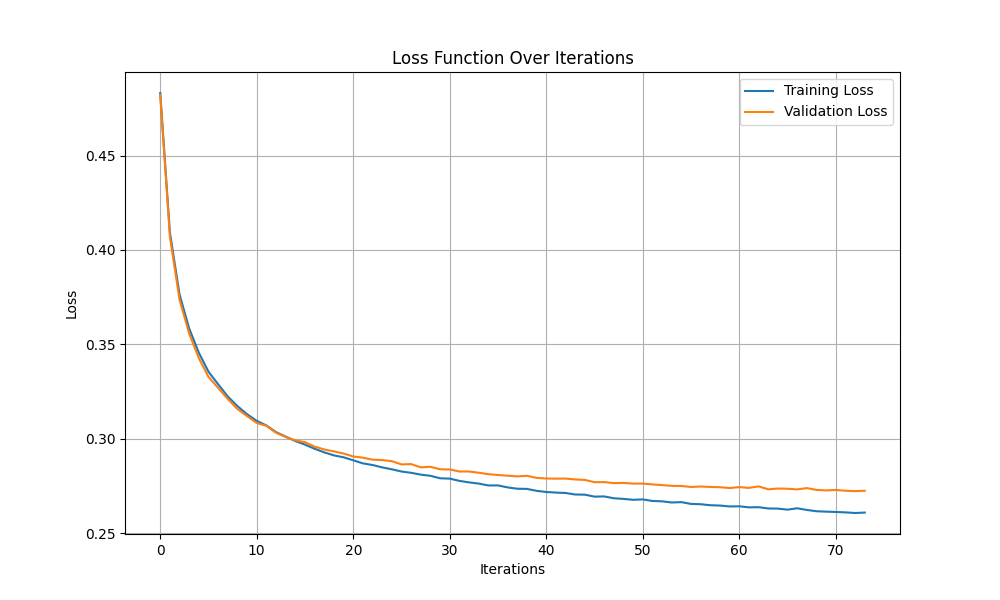
\includegraphics[width=0.8\linewidth]{img/lossfunction.png}
\caption{Training and validation loss over iterations.}
\label{fig:loss_curve}
\end{figure}

\subsection{Classification Performance}
Our model achieves an accuracy of approximately 92.5\% on the validation set and 92.37\% on the test set using the Adam optimizer. Table I shows the detailed results of our classification performance.

\begin{table}[htbp]
\caption{Classification Performance}
\begin{center}
\begin{tabular}{|c|c|}
\hline
\textbf{Metric} & \textbf{Value} \\
\hline
Validation Accuracy & 92.5\% \\
\hline
Test Accuracy & 92.37\% \\
\hline
\end{tabular}
\end{center}
\label{tab:performance}
\end{table}

\subsection{Confusion Matrix Analysis}
Fig. 2 shows the confusion matrix for the test set predictions. The diagonal elements represent the number of correctly classified instances for each class, while the off-diagonal elements represent misclassifications.

\begin{figure}[htbp]
\centering
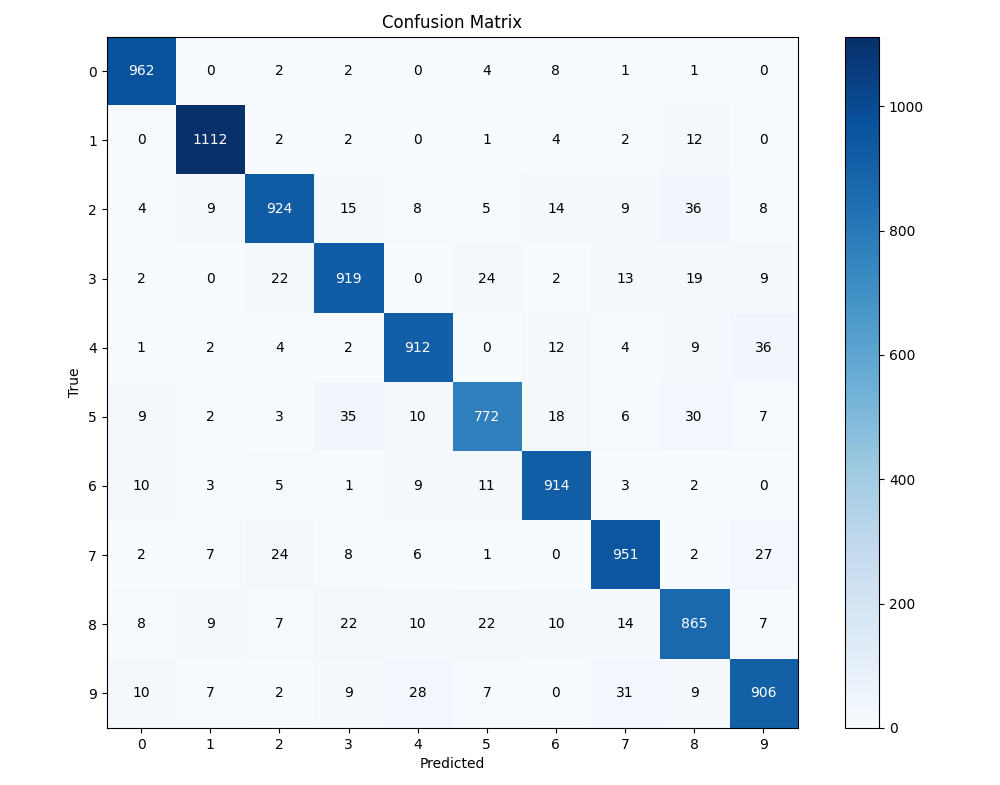
\includegraphics[width=0.8\linewidth]{img/confusionmatrix.png}
\caption{Confusion matrix for test set predictions.}
\label{fig:confusion_matrix}
\end{figure}

We observe that the majority of misclassifications occur between visually similar digits, such as:
\begin{itemize}
    \item 4 and 9, which share similar upper curves
    \item 3 and 5, which have similar structures
    \item 7 and 9, which can look similar with certain handwriting styles
\end{itemize}

These patterns highlight the limitations of linear models for image classification, as they cannot capture complex spatial patterns and relationships that deep learning models can learn.

\subsection{Sample Predictions}
Fig. 3 shows a sample of test images along with their true labels and model predictions. These examples provide a qualitative assessment of the model's performance and help identify patterns in correct and incorrect classifications.

\begin{figure}[htbp]
\centering
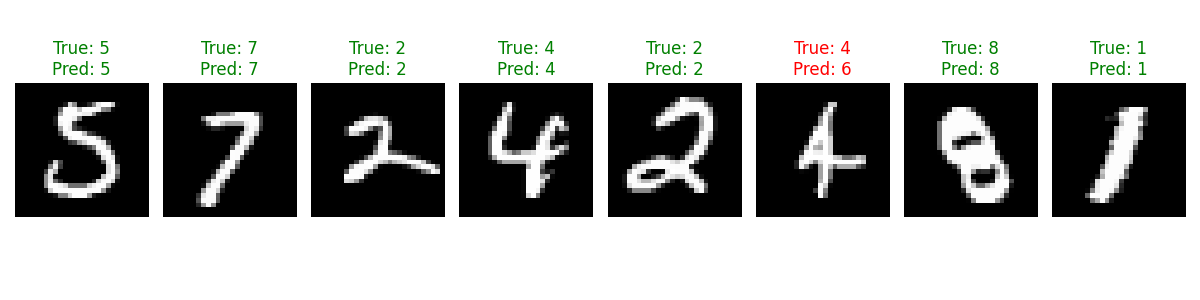
\includegraphics[width=0.8\linewidth]{img/output.png}
\caption{Sample test images with true labels and model predictions.}
\label{fig:sample_predictions}
\end{figure}

\subsection{Discussion}
Our results demonstrate that softmax regression can achieve reasonable performance on the MNIST dataset, despite being a linear model. The key observations from our experiments are:

\begin{itemize}
    \item \textbf{Effectiveness of Regularization:} L2 regularization helps prevent overfitting and improves generalization.
    
    \item \textbf{Learning Rate Decay:} The exponential decay of the learning rate helps the model converge more stably and achieve better performance.
    
    \item \textbf{Early Stopping:} Monitoring the validation loss and stopping training when it no longer improves helps prevent overfitting.
    
    \item \textbf{Limitations of Linear Models:} While softmax regression performs reasonably well, it cannot capture complex spatial patterns in the images. This limitation is evident in the misclassifications between visually similar digits.
\end{itemize}

\section{Implementation Details}
\subsection{Code Structure}
Our implementation consists of the following key components:

\begin{itemize}
    \item \textbf{Data Loading and Preprocessing:} Functions for loading data from CSV files, normalizing pixel values, and splitting the dataset.
    
    \item \textbf{Model Implementation:} Functions for softmax activation, cost computation, and gradient calculation.
    
    \item \textbf{Training Procedure:} Implementation of the Adam optimizer with learning rate adaptation and early stopping.
    
    \item \textbf{Evaluation:} Functions for computing accuracy, generating confusion matrices, and visualizing predictions.
\end{itemize}

\subsection{Softmax Function}
The softmax function is implemented as follows:

\begin{lstlisting}[language=Python]
def softmax(z):
    exp_z = np.exp(z - np.max(z, axis=1, keepdims=True))
    return exp_z / np.sum(exp_z, axis=1, keepdims=True)
\end{lstlisting}

Note that we subtract the maximum value of each row to prevent numerical overflow, which is a common issue when implementing the softmax function.

\subsection{Cost Function}
The cost function, including cross-entropy loss and L2 regularization, is implemented as follows:

\begin{lstlisting}[language=Python]
def compute_cost(X, y, w, b, lambda_=1):
    m = X.shape[0]
    z = np.dot(X, w) + b
    f_wb = softmax(z)
    cross_entropy_cost = -np.sum(y * np.log(f_wb + 1e-8)) / m
    
    regularization_cost = 0
    if lambda_ > 0:
        regularization_cost = (lambda_ / (2 * m)) * np.sum(np.square(w))
    
    return cross_entropy_cost + regularization_cost
\end{lstlisting}

\subsection{Gradient Computation}
The gradients of the cost function with respect to the parameters are computed as follows:

\begin{lstlisting}[language=Python]
def compute_gradient(X, y, w, b, lambda_=0):
    m = X.shape[0]
    z = np.dot(X, w) + b
    f_wb = softmax(z)
    error = f_wb - y
    
    dj_dw = np.dot(X.T, error) / m
    
    if lambda_ > 0:
        dj_dw += (lambda_ / m) * w
        
    dj_db = np.sum(error, axis=0) / m
    return dj_db, dj_dw
\end{lstlisting}

\subsection{Gradient Descent with Early Stopping}
The training procedure, including the Adam optimizer, mini-batch processing, and early stopping, is implemented as follows:

\begin{lstlisting}[language=Python]
def adam_optimizer(X, y, X_val, y_val, w_in, b_in, cost_function, gradient_function, 
                  alpha, num_iters, batch_size, lambda_, beta1=0.9, beta2=0.999,
                  epsilon=1e-8, patience=5, min_delta=0.001):
    m = X.shape[0]
    J_history = []
    val_history = []
    w_history = []
    
    # Initialize Adam parameters
    v_dw = np.zeros_like(w_in)
    v_db = np.zeros_like(b_in)
    s_dw = np.zeros_like(w_in)
    s_db = np.zeros_like(b_in)
    
    best_val_cost = float('inf')
    best_w = None
    best_b = None
    patience_counter = 0
    
    for i in range(num_iters):
        indices = np.random.permutation(m)
        X_shuffled = X[indices]
        y_shuffled = y[indices]
        
        for j in range(0, m, batch_size):
            t = i * (m // batch_size) + (j // batch_size) + 1
            
            X_batch = X_shuffled[j:j+batch_size]
            y_batch = y_shuffled[j:j+batch_size]
            
            # Compute gradients
            dj_db, dj_dw = gradient_function(X_batch, y_batch, w_in, b_in, lambda_)
            
            # Update momentum
            v_dw = beta1 * v_dw + (1 - beta1) * dj_dw
            v_db = beta1 * v_db + (1 - beta1) * dj_db
            
            # Update RMSprop
            s_dw = beta2 * s_dw + (1 - beta2) * np.square(dj_dw)
            s_db = beta2 * s_db + (1 - beta2) * np.square(dj_db)
            
            # Bias correction
            v_dw_corrected = v_dw / (1 - beta1**t)
            v_db_corrected = v_db / (1 - beta1**t)
            s_dw_corrected = s_dw / (1 - beta2**t)
            s_db_corrected = s_db / (1 - beta2**t)
            
            # Update parameters
            w_in -= alpha * (v_dw_corrected / (np.sqrt(s_dw_corrected) + epsilon))
            b_in -= alpha * (v_db_corrected / (np.sqrt(s_db_corrected) + epsilon))
        
        cost = cost_function(X, y, w_in, b_in, lambda_)
        J_history.append(cost)
        
        val_cost = cost_function(X_val, y_val, w_in, b_in, lambda_)
        val_history.append(val_cost)
        
        if i % (num_iters // 10) == 0 or i == num_iters - 1:
            w_history.append(w_in)
            print(f"Iteration {i:4}: Cost {cost:.4f}, Val Cost {val_cost:.4f}")
        
        # Early stopping
        if val_cost < best_val_cost - min_delta:
            best_val_cost = val_cost
            best_w = w_in.copy()
            best_b = b_in.copy()
            patience_counter = 0
        else:
            patience_counter += 1
            
        if patience_counter >= patience:
            print(f"Early stopping at iteration {i}")
            return best_w, best_b, J_history, val_history, w_history
    
    if best_w is not None:
        return best_w, best_b, J_history, val_history, w_history
    else:
        return w_in, b_in, J_history, val_history, w_history
\end{lstlisting}

\section{Conclusion}
In this paper, we presented a complete implementation of softmax regression for classifying handwritten digits in the MNIST dataset. Our approach incorporated the Adam optimizer, mini-batch processing, learning rate adaptation, and early stopping. Through detailed evaluation, we demonstrated the effectiveness of softmax regression for digit classification and analyzed its performance characteristics.

The experimental results show that:
\begin{itemize}
    \item Softmax regression can achieve competitive accuracy rates on the MNIST dataset
    \item The incorporation of regularization, learning rate decay, and early stopping significantly improves model performance
    \item Linear models have inherent limitations in capturing complex spatial patterns, leading to specific patterns of misclassification
\end{itemize}

Future work could explore:
\begin{itemize}
    \item Comparison with more complex models, such as neural networks and SVMs
    \item Feature engineering techniques to improve the performance of linear models
    \item Ensemble methods combining multiple softmax regression models
    \item Application to other multiclass classification problems
\end{itemize}

\section*{Acknowledgment}
The authors would like to thank the developers of NumPy and Matplotlib for providing the tools used in this implementation.

\end{document}